\chapter{Өгөгдөл ба туршилт}
\section{Туршилтын өгөгдөл}

Шаардлагад нийцсэн, синхрончлолын түвшин нь тэмдэглэгдсэн бодит олон хүний бичлэг олох боломж хязгаарлагдмал тул алгоритмыг голчлон хяналттай (синтетик) өгөгдөл дээр үнэлж, дараа нь бодит бичлэгүүд дээр шалгав. Хяналттай өгөгдлийн давуу тал нь хүмүүсийн хоорондох ялгааг (хоцрогдол, зай, байрлал гэх мэт) судлаач өөрөө тогтоодог тул алгоритмын үр дүнг жинхэнэ утгатай шууд харьцуулах боломжтой явдал юм.

\textbf{Хяналттай өгөгдөл үүсгэх арга.} Нэг хүний хөдөлгөөнийг агуулсан бичлэгийг эх сурвалж болгон авч, түүний хуулбарыг хоёр дахь хүн болгон эх бичлэгийн хажууд нь нэг кадрт зэрэгцүүлэн нийлүүлсэн. Иймд 1-р хүн (зүүн тал) нь эх бичлэг, 2-р хүн (баруун тал) нь өөрчилсөн хуулбар бөгөөд жинхэнэ хариу урьдчилан мэдэгдэнэ. Эх бичлэг нь нэг балетчны 13.9 секунд үргэлжлэх, 960×1080 нягтаршилтай, 30 кадр/с давтамжтай бичлэг бөгөөд тогтмол давтамжтай болгох үүднээс 25 кадр/с (347 кадр) руу хөрвүүлсэн. Балетын хөдөлгөөнд гар, хөл хоёулаа идэвхтэй оролцдог тул үений бүх өнцгийг шалгахад тохиромжтой. Хуулбарт хийсэн өөрчлөлтүүдийг FFmpeg программын шүүлтүүрүүдээр үүсгэсэн (Хүснэгт~\ref{tab:synthetic}).

\begin{table}[H]
\centering
\caption{Хяналттай өгөгдөл үүсгэсэн өөрчлөлтүүд}
\label{tab:synthetic}
\small
\begin{tabular}{|>{\raggedright\arraybackslash}p{0.150\linewidth}|>{\raggedright\arraybackslash}p{0.260\linewidth}|>{\raggedright\arraybackslash}p{0.230\linewidth}|>{\raggedright\arraybackslash}p{0.230\linewidth}|}
\hline
\textbf{Өөрчлөлт} & \textbf{Хэрхэн үүсгэсэн (FFmpeg)} & \textbf{Утгууд} & \textbf{Шалгасан зүйл} \\ \hline
Цагийн хоцрогдол & Хуулбарын эхэнд эхний кадрыг давтаж хойшлуулах (\texttt{tpad}) & 0, 1, 2, 3, 5, 8, 12, 25 кадр (0--1 секунд) & Хоцрогдол тодорхойлох нарийвчлал, онооны өөрчлөлт \\ \hline
Толин тусгал & Хуулбарыг хэвтээ чиглэлд эргүүлэх (\texttt{hflip}) & 0 ба 8 кадрын хоцрогдолтой & Хоёр горимт харьцуулалт \\ \hline
Өөр хөдөлгөөн & Хуулбарыг эх бичлэгийн өөр хэсгээс эхлүүлэх & 4, 7, 10 секундийн зөрүүтэй & Хоцрогдлын итгэлцлийн шалгалт \\ \hline
Камерын зай & Хуулбарыг жижигрүүлж доод талд нь байрлуулах (\texttt{scale}, \texttt{pad}) & 100, 75, 50, 25\%, 0 ба 8 кадрын хоцрогдолтой & Өнцөгт суурилсан арга зайнаас үл хамаарах эсэх \\ \hline
Нягтаршил & Хосын бичлэгийг багасгах (\texttt{scale}) & 1080p, 720p, 480p, 360p, 240p, 8 кадрын хоцрогдолтой & Гол цэг болон онооны тогтвортой байдал \\ \hline
Кадрын давтамж & 30 кадр/с хосын бичлэгийг бууруулах (\texttt{fps}) & 30, 25, 15, 10 кадр/с, 0.3 секундийн хоцрогдолтой & Хоцрогдлын нарийвчлал \\ \hline
Хүний тоо & Эх бичлэгийн 2, 3, 4 хуулбарыг зэрэгцүүлэх, сүүлийнхийг хоцроох & 2, 3, 4 хүн, 8 кадрын хоцрогдолтой & Бүлгээсээ зөрж буй хүнийг илрүүлэх, хурд \\ \hline
\end{tabular}
\end{table}

Байрлалын шилжилтийг тусад нь шалгаагүй. Учир нь үений өнцөг нь кадр дахь байрлалаас математикийн хувьд хамааралгүй бөгөөд хосын бичлэг бүрт хоёр хүн аль хэдийн кадрын өөр хэсэгт байрладаг.

\textbf{Гол цэгийн түвшний хяналттай өгөгдөл.} Видеог дахин боловсруулахгүйгээр алгоритмыг HPE-ийн алдаанаас тусгаарлан шалгахын тулд бодит бичлэгийн гол цэгийн цуваанд шууд өөрчлөлт оруулав. Тухайлбал, нэг хүний бүх бие эсвэл нэг, хоёр мөчийн гол цэгийг тодорхой хугацаанд хоцроох, мөн тухайн хүний хөдөлгөөнийг бичлэгийн өөр хэсгийнхээр солих.

\textbf{Бодит бичлэг.} Бодит нөхцөлд шалгахдаа загвар сонголтын бичлэг (гурван хүн тулааны урлагийн ижил хөдөлгөөн хийсэн, 720×1280, 25 кадр/с, 856 кадр) болон гурван бүжигчин хамтдаа бүжиглэсэн дөрвөн бичлэгийг (1920×1080, 59.94 кадр/с, 31--43 секунд) ашигласан. Эдгээр бичлэгийн синхрончлолын жинхэнэ түвшин тэмдэглэгдээгүй тул үр дүнг чанарын хувьд тайлбарлав.

\textbf{Боловсруулалт.} Хяналттай болон бодит бүх бичлэгийг RTMPose-m загвараар (хүн илрүүлэгчийн итгэлцлийн босго 0.25) HPE серверт (CUDA, NVIDIA GeForce RTX 2060) боловсруулж, синхрончлолыг хувилбар 2-ын анхдагч тохиргоогоор тооцоолсон. Бичлэг үүсгэх, серверт боловсруулах, оноо тооцоолж CSV файлд хадгалах бүх алхмыг нэг скриптээр автоматжуулсан тул туршилтыг бүхэлд нь дахин гүйцэтгэх боломжтой.

\section{Үнэлгээний хэмжүүрүүд}

\begin{table}[H]
\centering
\caption{Үнэлгээний хэмжүүрүүд}
\label{tab:metrics}
\small
\begin{tabular}{|>{\raggedright\arraybackslash}p{0.234\linewidth}|>{\raggedright\arraybackslash}p{0.260\linewidth}|>{\raggedright\arraybackslash}p{0.372\linewidth}|}
\hline
\textbf{Хэмжүүр} & \textbf{Юуг үнэлэх} & \textbf{Сайн үр дүн} \\ \hline
Нөхцөл хоорондын ялгаа & Синхрон, хоцрогдолтой, өөр хөдөлгөөнтэй бичлэгүүдийн оноо зөв дараалалд ялгарч буйг & Синхрон \textgreater{} хоцрогдолтой \textgreater{} өөр хөдөлгөөн \\ \hline
Онооны тогтвортой байдал & Ижил нөхцөлтэй бичлэгүүдийн оноо хэр ойролцоо гарч буйг & Бага зөрүү \\ \hline
Хоцрогдлын алдаа (мс) & Тооцоолсон хоцрогдол жинхэнэ хоцрогдлоос хэр зөрж буйг & 0-д ойр \\ \hline
Гол цэгийн тохирол (PCK@0.05) & Нягтаршил буурахад гол цэг жишиг бичлэгийнхээс хэр зөрж буйг & 100\%-д ойр \\ \hline
Боловсруулалтын хурд & Нэг кадрын хугацаа (мс), бодит хурд (кадр/с) & Бага хугацаа \\ \hline
\end{tabular}
\end{table}

\headshort{Хөтөч ба сервер}
\section{Вэб хөтөч ба серверийн боловсруулалт}

Загвар сонголтын бичлэгийг (856 кадр, 25 кадр/с) RTMPose-m загвараар вэб хөтөч дээр (WebGPU) болон сервер дээр (CUDA) боловсруулж харьцуулав (Хүснэгт~\ref{tab:browser_server}, Зураг~\ref{fig:fig7_browser_vs_server}).

\begin{table}[H]
\centering
\caption{Вэб хөтөч ба серверийн боловсруулалтын харьцуулалт}
\label{tab:browser_server}
\small
\begin{tabular}{|>{\raggedright\arraybackslash}p{0.420\linewidth}|>{\raggedright\arraybackslash}p{0.220\linewidth}|>{\raggedright\arraybackslash}p{0.220\linewidth}|}
\hline
\textbf{Үзүүлэлт} & \textbf{Вэб хөтөч} & \textbf{Сервер} \\ \hline
Тооцооллын төхөөрөмж & WebGPU & CUDA \\ \hline
Нэг кадрын хугацаа, дундаж (мс) & 113.8 & 50.8 \\ \hline
Нэг кадрын хугацаа, 95-р перцентиль (мс) & 160.3 & 83.8 \\ \hline
Бодит хурд (кадр/с) & 5.5 & 17.4 \\ \hline
Гурван хүн бүгд илэрсэн кадр & 100\% & 100\% \\ \hline
Гурваас олон хүн илэрсэн кадр & 3.0\% & 4.0\% \\ \hline
Гол цэгийн дундаж итгэлцэл & 0.709 & 0.711 \\ \hline
Чичиргээ (хүрээний өндрийн \%) & 1.46 & 1.48 \\ \hline
Мөчдийн уртын хэлбэлзэл (\%) & 18.7 & 18.9 \\ \hline
Бүлгийн синхрончлолын оноо & 82.6 & 81.4 \\ \hline
\end{tabular}
\end{table}

Серверийн бодит хурдад видео илгээх (0.1 секунд) болон боловсруулалтын хугацааг оруулсан бөгөөд хөтөч дээр араг яс зурах, видео кодчилох хугацаа мөн орсон. Сервер вэб хөтчөөс 2.2 дахин хурдан ажилласан. Хоёр горимд ижил хүмүүсийн гол цэгүүдийн хоорондох зай медианаар 0.61 пиксел, 95-р перцентилээр 2.25 пиксел, дунджаар хүний хүрээний өндрийн 0.29\% байв. Кадруудын 98.6\%-д илэрсэн хүний тоо ижил байсан бөгөөд аль ч горимд гурваас цөөн хүн илэрсэн кадр байгаагүй тул ялгаа нь гурваас олон хүн илэрсэн (26 ба 34) кадруудад гарсан. Ийм бага зөрүү нь хоёр орчинд видео задлах (OpenCV ба вэб хөтөч) болон зургийн хэмжээ өөрчлөх аргын ялгаанаас гарна. Харин бүлгийн синхрончлолын оноо 1.2 оноогоор зөрсөн бөгөөд шалтгааныг 4.4-т тайлбарлав.

\begin{figure}[H]
\centering
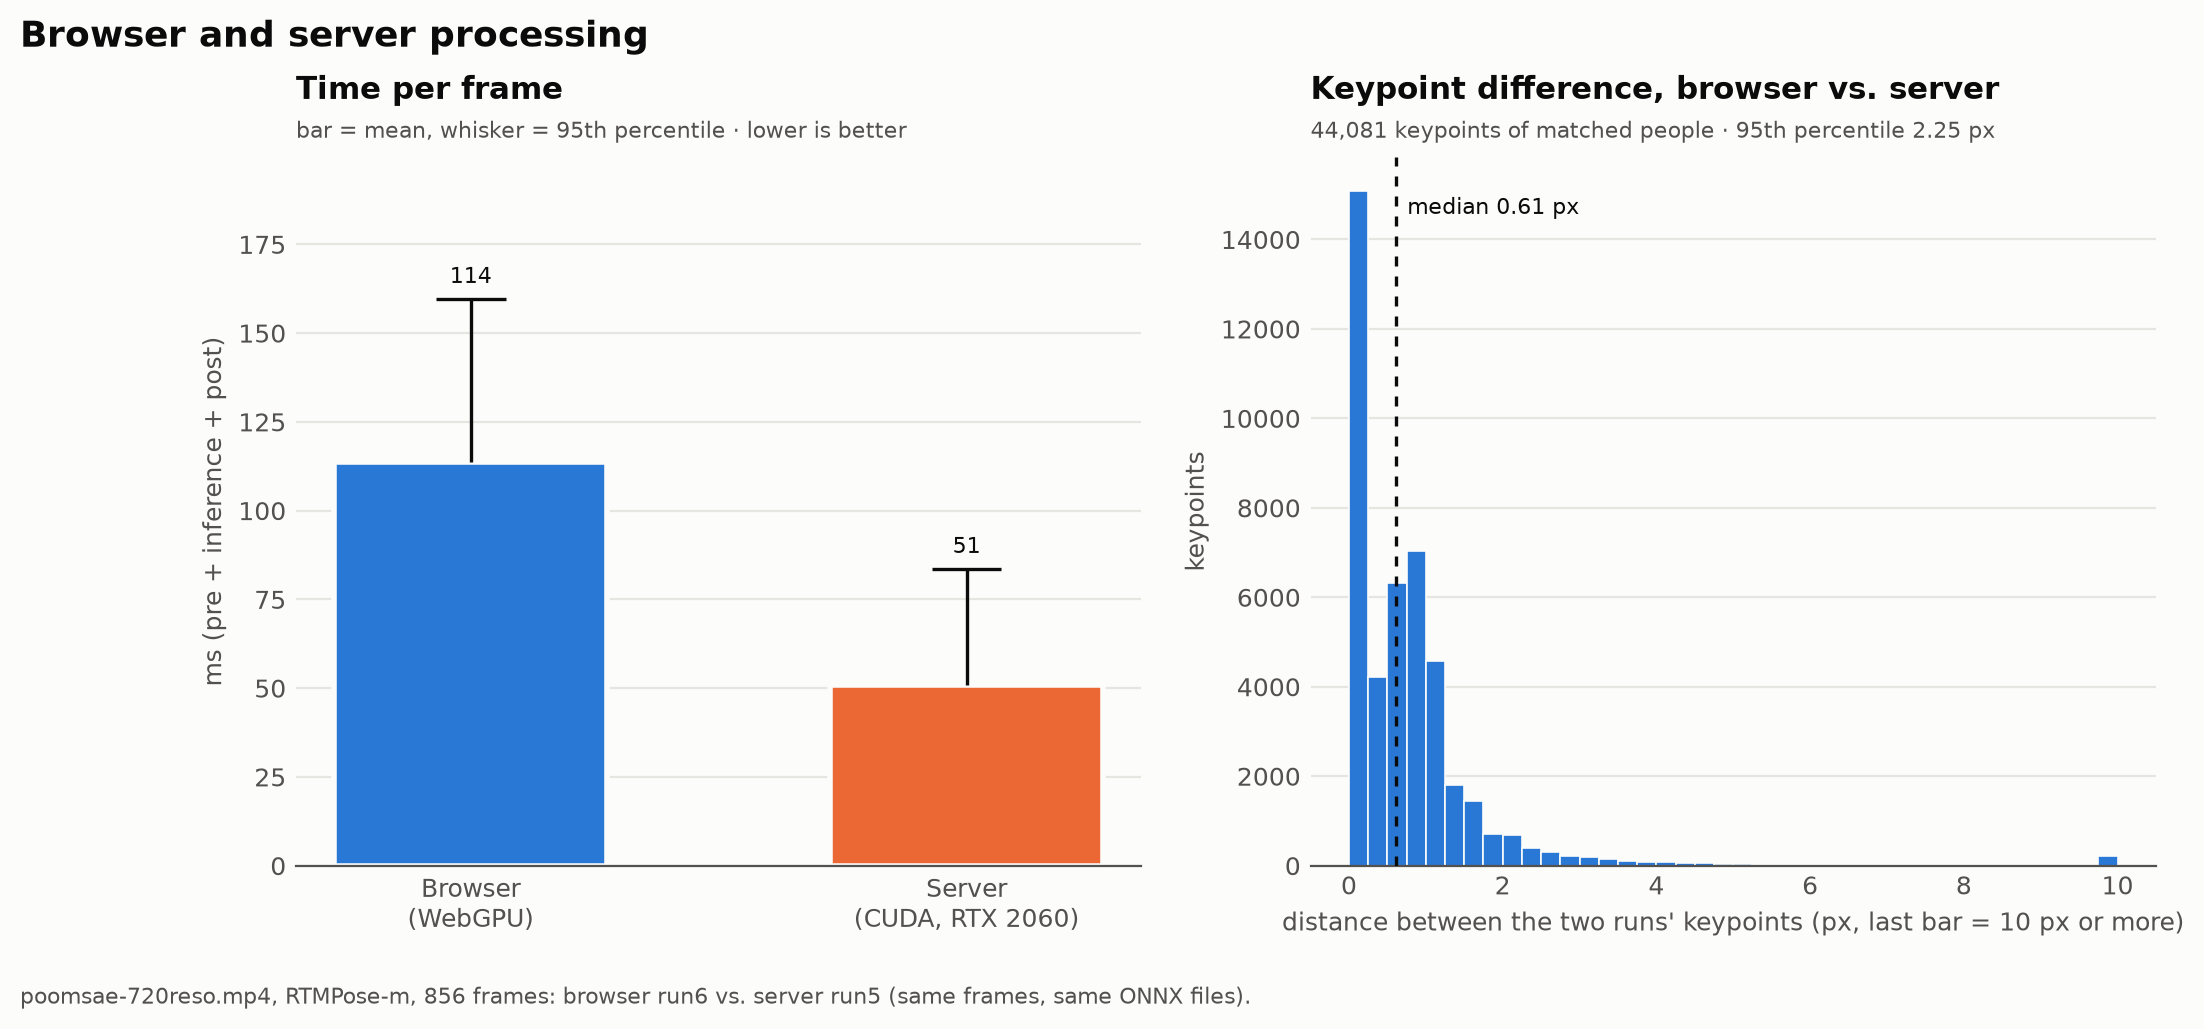
\includegraphics[width=\linewidth]{fig7_browser_vs_server}
\caption{Вэб хөтөч ба серверийн нэг кадрын хугацаа болон гол цэгийн зөрүүний тархалт}
\label{fig:fig7_browser_vs_server}
\end{figure}

\textbf{Кадр унших алдаа ба түүний засвар.} Хоёр горимыг харьцуулах явцад вэб хөтчийн кадр унших аргад алдаа илэрсэн. Анхны хэрэгжүүлэлтэд i-р кадрыг уншихдаа видеог яг \(i/f\) хугацаа руу шилжүүлдэг байв. Кадрын яг хил дээр шилжихэд Chrome хөтөч заримдаа өмнөх кадрыг харуулдаг тул 30 кадр/с давтамжтай бичлэгт уншсан кадрын дугаарууд 0, 1, 1, 3, 4, 4, 6, \ldots{} буюу гурван кадр тутмын нэг нь давхардаж, нэг нь алгасагдаж байв. Мөн эхний кадрын цагийн тэмдэг нь 0.04 секунд байсан загвар сонголтын бичлэгт бүх кадр нэг кадраар хоцорч, 856 кадрын оронд 858 кадр боловсруулагдсан. Засварын дараа видеог кадрын голд, өөрөөр хэлбэл эхний кадрын цагийн тэмдэг \(+ (i + 0.5)/f\) хугацаа руу шилжүүлдэг болсноор i-р ажиллуулалтын кадр нь видеоны жинхэнэ i-р кадртай тохирч, сервер ч мөн ижил кадруудыг уншдаг болсон. Энэ засвараас өмнө хийсэн 3.2-ын загваруудын харьцуулалт болон загвар бүрийн нягтаршлын туршилтад энэ алдаа нөлөөлсөн. Бүх загвар ижил аргаар хэмжигдсэн тул загваруудын харьцангуй дүгнэлт хүчинтэй боловч чичиргээний үнэмлэхүй утга бага зэрэг өөр байж болзошгүй. Энэ бүлгийн бусад бүх туршилтыг засварын дараа серверээр хийсэн тул алдаанд өртөөгүй.

\headshort{Алгоритмын туршилт}
\section{Синхрончлолын алгоритмын туршилт}

\textbf{Цагийн хоцрогдол.} Хуулбарыг 0--25 кадраар (0--1 секунд) хоцроосон найман бичлэг дээр алгоритм бүх бичлэгийн хоцрогдлыг найман тохиолдол бүгдэд нь яг зөв, өөрөөр хэлбэл 0 мс алдаатай олсон (Хүснэгт~\ref{tab:lag_test}, Зураг~\ref{fig:fig11_lag}). Хамгийн их корреляц \(\rho_{max}\) бүх тохиолдолд 0.95-аас их тул олдсон хоцрогдол бүгд найдвартай гэж тэмдэглэгдсэн.

\begin{table}[H]
\centering
\caption{Видеоны түвшний хоцрогдлын туршилтын үр дүн (1--2 хос)}
\label{tab:lag_test}
\small
\begin{tabular}{|>{\raggedright\arraybackslash}p{0.110\linewidth}|>{\raggedright\arraybackslash}p{0.105\linewidth}|>{\raggedright\arraybackslash}p{0.085\linewidth}|>{\raggedright\arraybackslash}p{0.085\linewidth}|>{\raggedright\arraybackslash}p{0.085\linewidth}|>{\raggedright\arraybackslash}p{0.085\linewidth}|>{\raggedright\arraybackslash}p{0.110\linewidth}|>{\raggedright\arraybackslash}p{0.085\linewidth}|}
\hline
\textbf{Хоцрогдол (кадр)} & \textbf{Жинхэнэ (с)} & \(S\) & \(S_{pose}\) & \(S_{corr}\) & \(S_{lag}\) & \textbf{Олдсон (с)} & \(\rho_{max}\) \\ \hline
0 & 0 & 99.8 & 0.996 & 0.998 & 1.000 & 0 & 0.98 \\ \hline
1 & 0.04 & 97.1 & 0.968 & 0.972 & 0.974 & 0.04 & 0.96 \\ \hline
2 & 0.08 & 93.1 & 0.939 & 0.906 & 0.947 & 0.08 & 0.97 \\ \hline
3 & 0.12 & 89.0 & 0.916 & 0.832 & 0.921 & 0.12 & 0.97 \\ \hline
5 & 0.20 & 80.9 & 0.879 & 0.681 & 0.868 & 0.20 & 0.97 \\ \hline
8 & 0.32 & 71.8 & 0.839 & 0.525 & 0.789 & 0.32 & 0.99 \\ \hline
12 & 0.48 & 64.4 & 0.812 & 0.436 & 0.684 & 0.48 & 0.96 \\ \hline
25 & 1.00 & 54.3 & 0.798 & 0.485 & 0.344 & 1.00 & 0.95 \\ \hline
\end{tabular}
\end{table}

\begin{figure}[H]
\centering
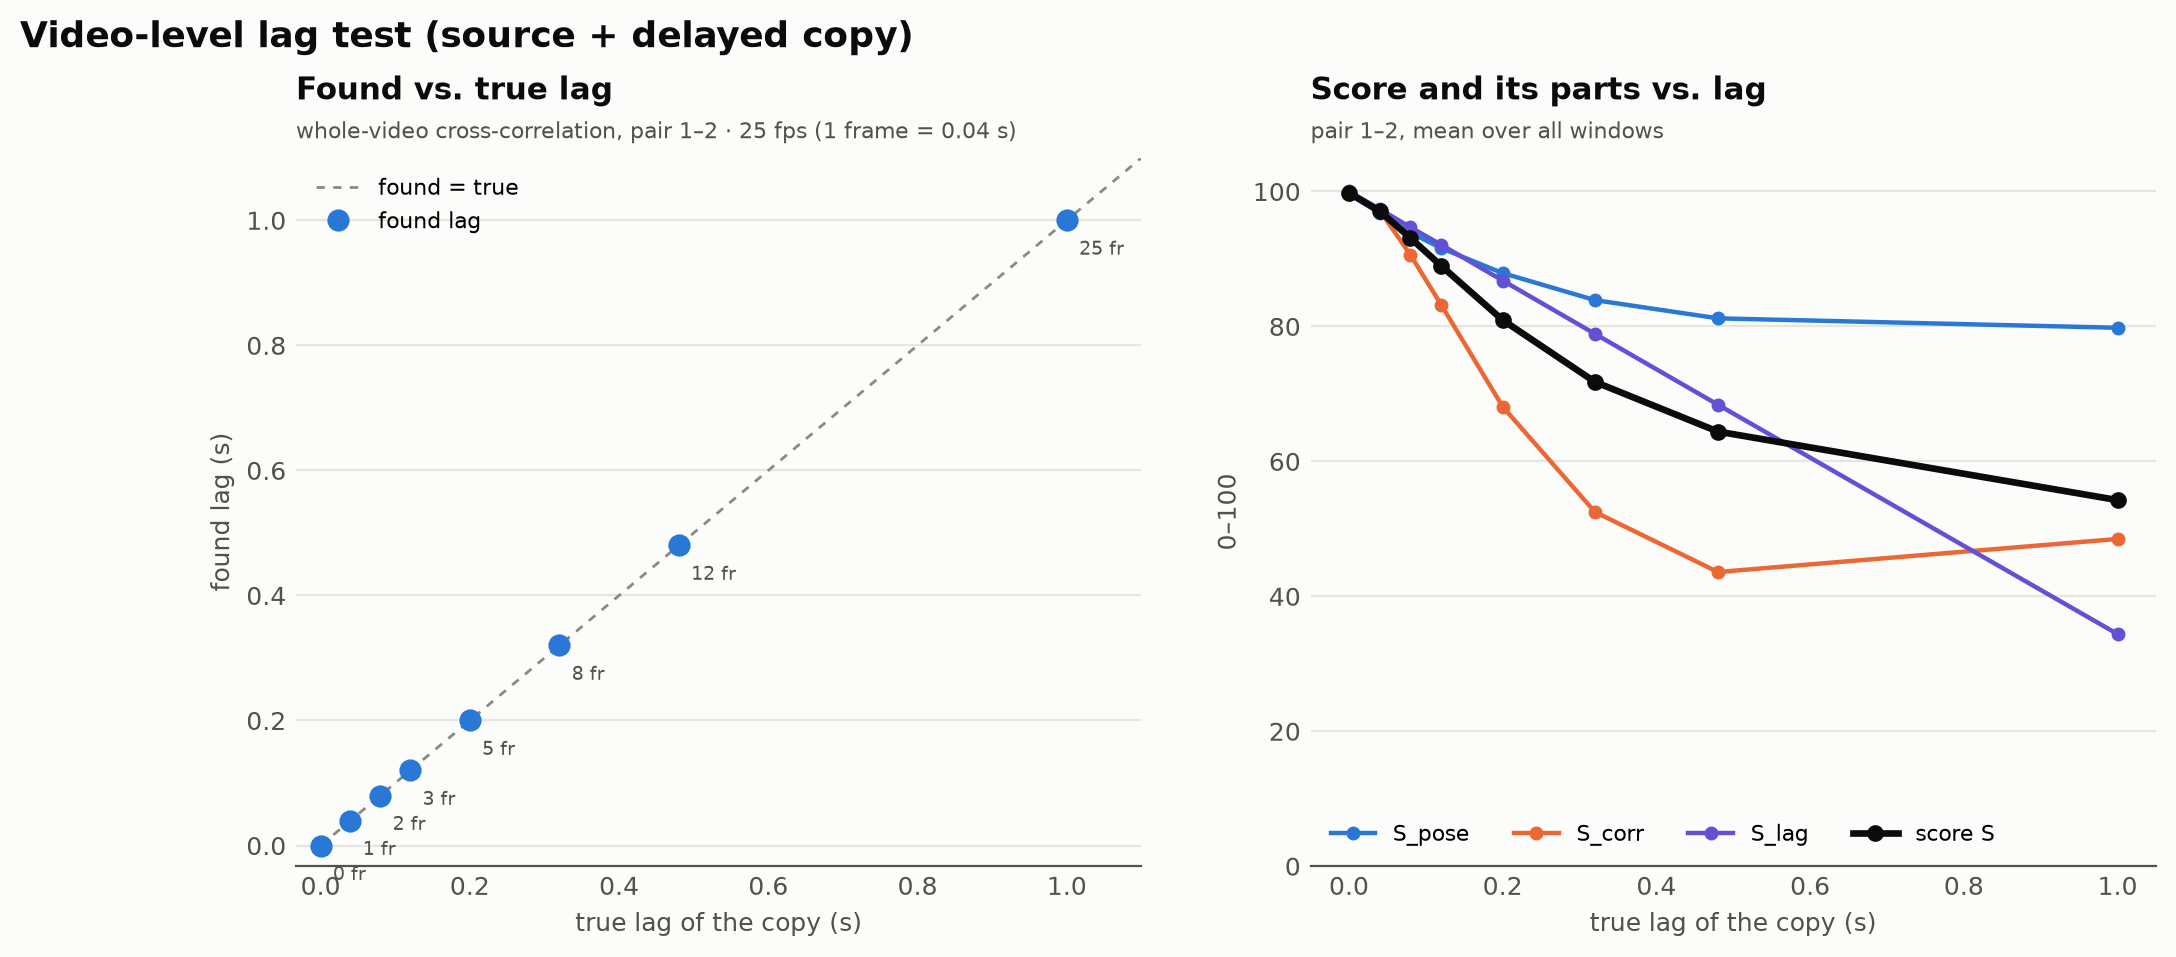
\includegraphics[width=\linewidth]{fig11_lag}
\caption{Олдсон ба жинхэнэ хоцрогдол, мөн хоцрогдлоос хамаарах оноо ба түүний бүрэлдэхүүнүүд}
\label{fig:fig11_lag}
\end{figure}

Хоцрогдол нэмэгдэх тусам нэгдсэн оноо 99.8-аас 54.3 хүртэл жигд буурсан. Бүрэлдэхүүн тус бүрээр авч үзвэл хөдөлгөөний уялдаа \(S_{corr}\) хамгийн мэдрэмтгий бөгөөд 0.2 секундийн хоцрогдолд 0.68 хүртэл буурсан бол байрлалын ижил төстэй байдал \(S_{pose}\) аажуухан буурч, 0.48 секундээс хойш бараг тогтмол болсон. Хоцрогдлын оноо \(S_{lag}\) нь \(1 - |\tau^{*}|/\tau_{max}\) томьёоны дагуу шугаман буурсан. Синхрончлол алдагдсан мөч нь 0.2 секунд ба түүнээс их хоцрогдолтой бичлэгүүдэд бүх бичлэгийг хамарч, зөв хоцрогдолтойгоор илэрсэн бөгөөд 0.12 секундээс бага хоцрогдолд илрээгүй нь «хоцорсон» гэж тооцох анхдагч 0.2 секундийн босготой тохирч байна.

\textbf{Толин тусгал ба өөр хөдөлгөөн.} Хэвтээ чиглэлд эргүүлсэн хуулбарын хувьд цонхнуудын 100\%-д толин тусгал горим сонгогдож, оноо 99.3 буюу синхрон бичлэгтэй бараг тэнцүү гарсан. Толин тусгал хуулбарыг 8 кадраар хоцроосон үед оноо 71.5 болж, хоцрогдол мөн 0.32 секунд гэж зөв олдсон. Харин эх бичлэгийн өөр хэсгийн хөдөлгөөнөөр солиход оноо 4, 7, 10 секундийн зөрүүд харгалзан 62.0, 53.7, 45.4 болж буурсан бөгөөд бүх тохиолдолд \(\rho_{max}\) нь 0.11--0.22 буюу \(\rho_{min} = 0.3\)-аас бага тул бүх бичлэгийн хоцрогдлыг найдваргүй гэж зөв тэмдэглэсэн (Зураг~\ref{fig:fig12_conditions}).

\begin{figure}[H]
\centering
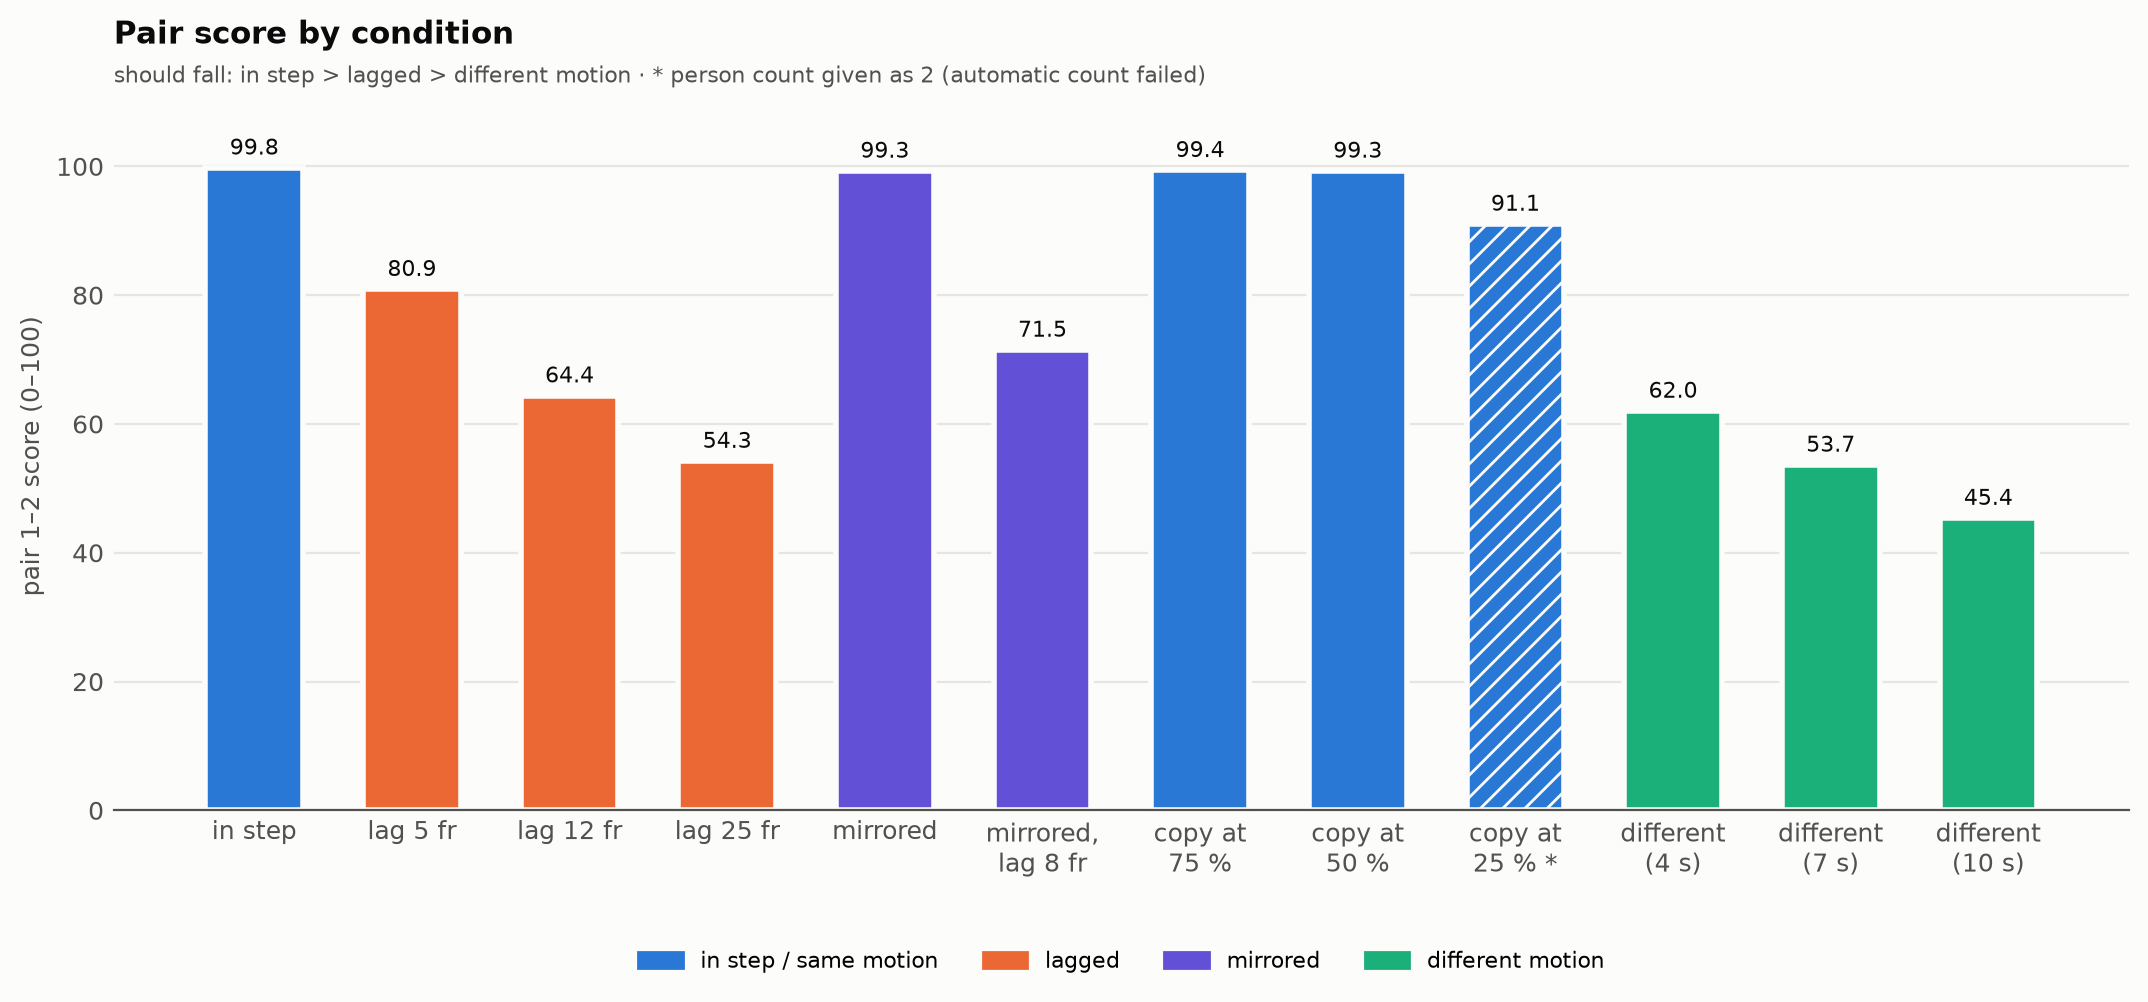
\includegraphics[width=\linewidth]{fig12_conditions}
\caption{Нөхцөл тус бүрийн 1--2 хосын оноо}
\label{fig:fig12_conditions}
\end{figure}

Нөхцлүүдийн оноо синхрон (99.3--99.8) \(>\) 0.2--0.5 секундийн хоцрогдолтой (64.4--80.9) \(>\) өөр хөдөлгөөн (45.4--62.0) гэсэн хүлээгдэж буй дарааллаар ялгарсан. Гэвч 1 секундийн хоцрогдолтой бичлэгийн оноо (54.3) нь 4 секундийн зөрүүтэй өөр хөдөлгөөний онооноос (62.0) бага гарсан. Энэ нь 1 секунд орчим ба түүнээс их хоцрогдол оноогоороо өөр хөдөлгөөнтэй ижил түвшинд хүрдгийг харуулах бөгөөд ийм тохиолдолд хоёрыг ялгахад бүх бичлэгийн хоцрогдол болон \(\rho_{max}\)-ийг хамт харах шаардлагатай. Хоцрогдлын хувьд 1 секундийн тохиолдолд \(\rho_{max} = 0.95\) байсан бол өөр хөдөлгөөнд 0.11--0.22 байсан тул энэ хоёр үзүүлэлтээр тэдгээрийг тод ялгах боломжтой.

\textbf{Камерын зай, нягтаршил, кадрын давтамж.} Оролтын бичлэгийн шинж чанарын нөлөөг Хүснэгт~\ref{tab:robustness} болон Зураг~\ref{fig:fig13_robustness}-д нэгтгэв.

\begin{table}[H]
\centering
\caption{Оролтын бичлэгийн шинж чанарын нөлөө (1--2 хос)}
\label{tab:robustness}
\small
\begin{tabular}{|>{\raggedright\arraybackslash}p{0.280\linewidth}|>{\raggedright\arraybackslash}p{0.100\linewidth}|>{\raggedright\arraybackslash}p{0.170\linewidth}|>{\raggedright\arraybackslash}p{0.140\linewidth}|>{\raggedright\arraybackslash}p{0.150\linewidth}|}
\hline
\textbf{Нөхцөл} & \textbf{Оноо} & \textbf{Олдсон хоцрогдол (алдаа)} & \textbf{PCK@0.05} & \textbf{Хоёр хүн илэрсэн кадр} \\ \hline
Хуулбар 100\%, синхрон & 99.8 & 0 с (0 мс) & -- & 345/347 \\ \hline
Хуулбар 75\%, синхрон & 99.4 & 0 с (0 мс) & -- & 345/347 \\ \hline
Хуулбар 50\%, синхрон & 99.3 & 0 с (0 мс) & -- & 324/347 \\ \hline
Хуулбар 25\%, синхрон & 91.1* & 0 с (0 мс)* & -- & 114/347 \\ \hline
Хуулбар 75\%, 8 кадр & 71.8 & 0.32 с (0 мс) & -- & 344/347 \\ \hline
Хуулбар 50\%, 8 кадр & 71.8 & 0.32 с (0 мс) & -- & 321/347 \\ \hline
Хуулбар 25\%, 8 кадр & 71.4* & 0.32 с (0 мс)* & -- & 129/347 \\ \hline
1080p, 8 кадр & 71.8 & 0.32 с (0 мс) & 100\% & 344/347 \\ \hline
720p, 8 кадр & 71.6 & 0.32 с (0 мс) & 99.6\% & 344/347 \\ \hline
480p, 8 кадр & 71.5 & 0.32 с (0 мс) & 99.2\% & 344/347 \\ \hline
360p, 8 кадр & 71.6 & 0.32 с (0 мс) & 99.4\% & 344/347 \\ \hline
240p, 8 кадр & 71.4* & 0.32 с (0 мс)* & 98.5\% & 81/347 \\ \hline
30 кадр/с, 0.3 с & 73.0 & 0.30 с (0 мс) & -- & -- \\ \hline
25 кадр/с, 0.3 с & 73.3 & 0.28 с (20 мс) & -- & -- \\ \hline
15 кадр/с, 0.3 с & 73.3 & 0.27 с (33 мс) & -- & -- \\ \hline
10 кадр/с, 0.3 с & 73.0 & 0.30 с (0 мс) & -- & -- \\ \hline
\end{tabular}
\end{table}

\begin{figure}[H]
\centering
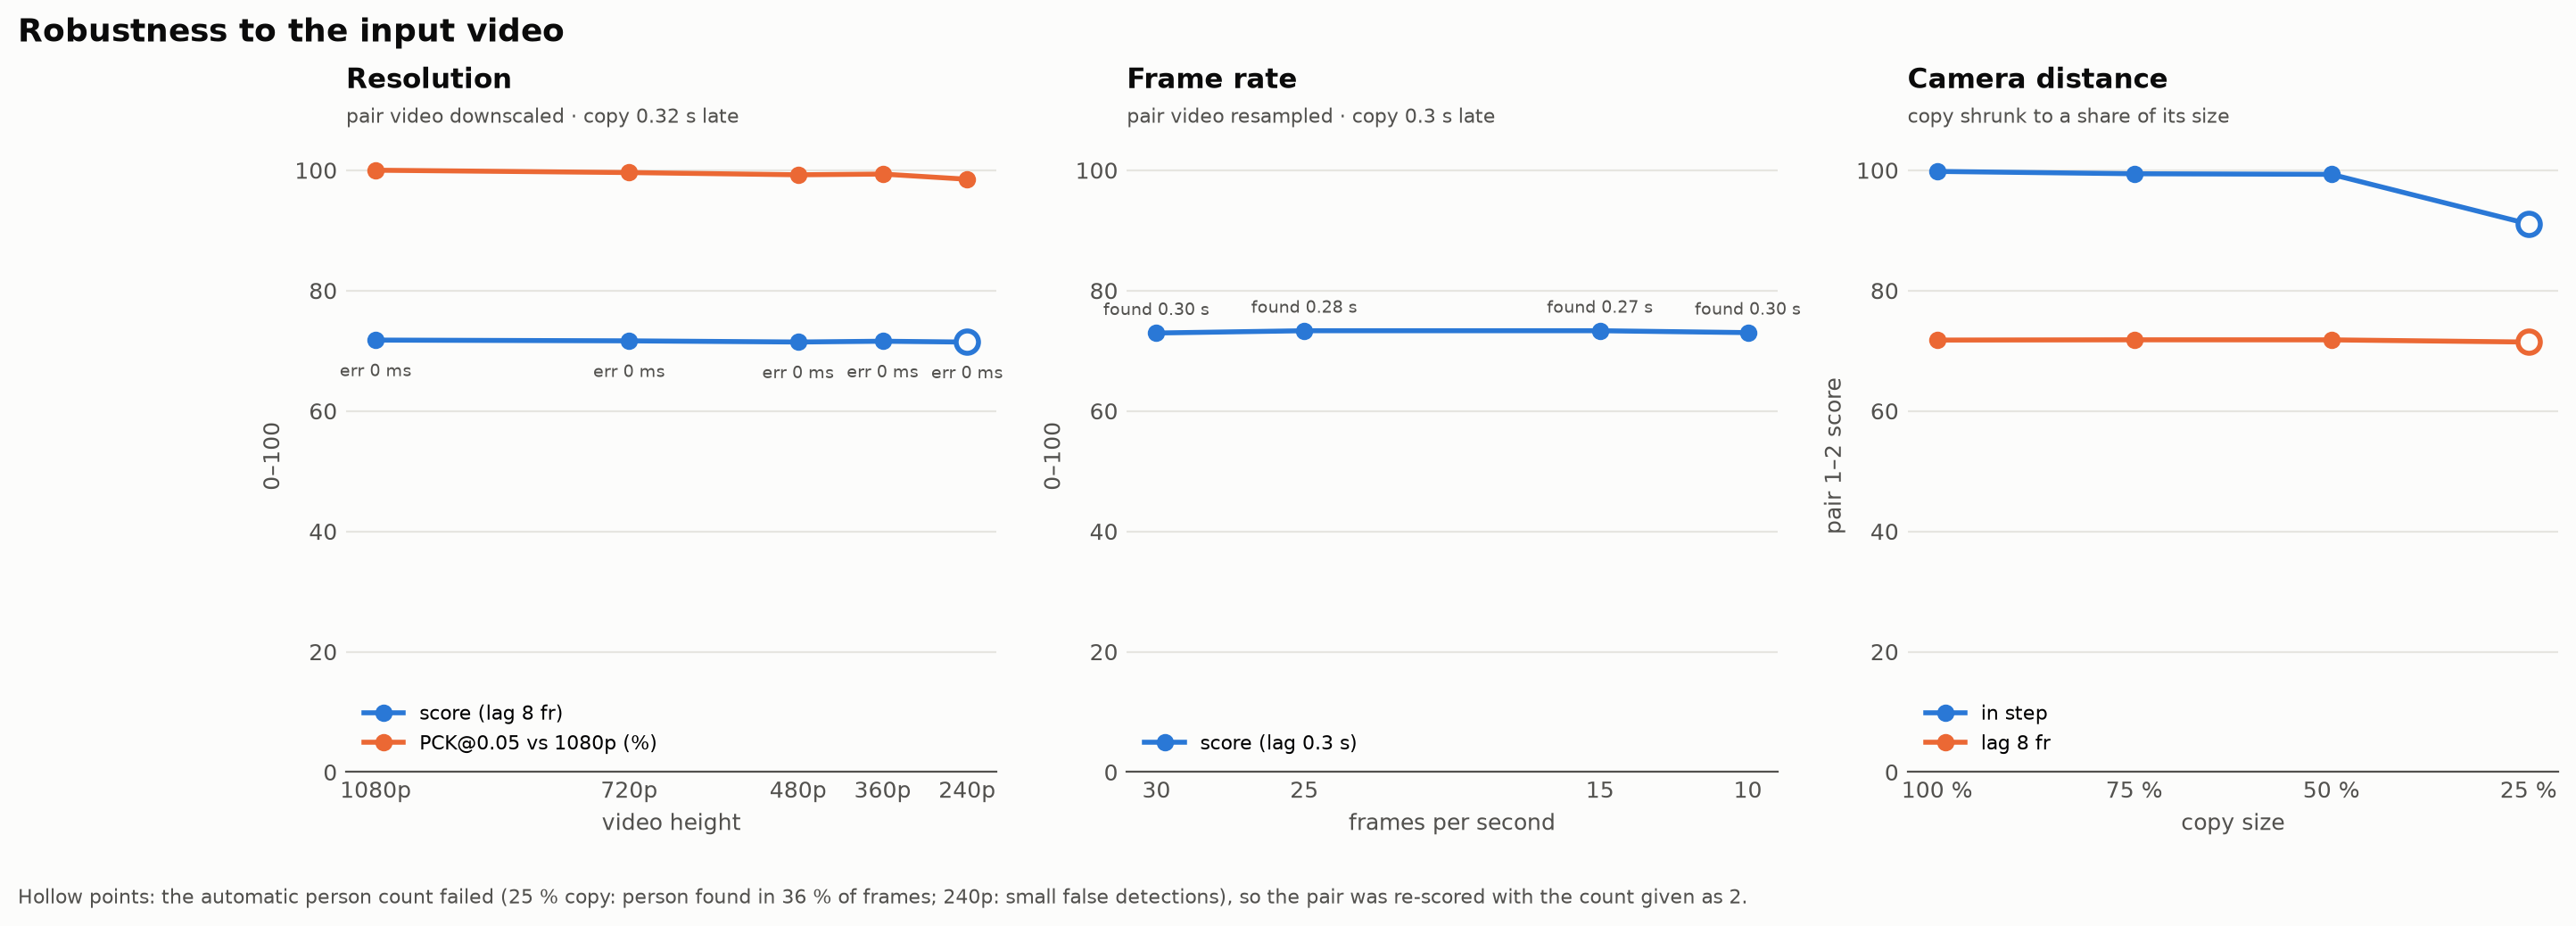
\includegraphics[width=\linewidth]{fig13_robustness}
\caption{Нягтаршил, кадрын давтамж болон камерын зайн нөлөө}
\label{fig:fig13_robustness}
\end{figure}

Хуулбарыг 50\% хүртэл жижигрүүлэхэд оноо 99.8-аас 99.3 болж бараг өөрчлөгдөөгүй нь үений өнцөгт суурилсан арга хүний зураг дээрх хэмжээнээс хамааралгүй болохыг баталж байна. Нягтаршлыг 1080p-ээс 360p хүртэл бууруулахад гол цэгийн 99.2\%-иас дээш нь жишиг байрлалынхаа хүрээний өндрийн 5\%-ийн дотор үлдэж, оноо 71.5--71.8, хоцрогдлын алдаа 0 мс байв. Кадрын давтамжийг 10 кадр/с хүртэл бууруулахад хоцрогдлын алдаа 0--33 мс буюу тухайн давтамжийн нэг кадрын хугацаанаас (33--100 мс) бага байсан бөгөөд оноо 73.0--73.3 хооронд тогтвортой байв.

Хоёр тохиолдолд хүний тоог автоматаар тодорхойлох алхам алдаа гаргасан (Хүснэгт~\ref{tab:robustness}-ийн * тэмдэгтэй мөрүүд). Хуулбарыг 25\% хүртэл жижигрүүлэхэд (хүний өндөр ойролцоогоор 140 пиксел) хүн илрүүлэгч жижиг хүнийг кадруудын ердөө 36\%-д илрүүлсэн тул эхний 2 секундэд хамгийн олон давтагдсан илрүүлэлтийн тоо 1 болж, хос үүсээгүй. 240p нягтаршилд жижиг, итгэлцэл багатай худал илрүүлэлтүүд олон гарч хүний тоо 4 гэж тоологдсон. Хүний тоог 2 гэж гараар өгөхөд хоёр тохиолдолд хоцрогдол зөв олдож, оноо нь бусад нөхцөлтэй ойролцоо гарсан. Харин 25\%-ийн синхрон бичлэгийн оноо (91.1) бусдаас бага байгаа нь 2-р хүн кадруудын 64\%-д илрээгүй, нөхөгдөх боломжгүй урт завсар үүссэнтэй холбоотой. Иймд хүний өндөр 140 пикселээс бага эсвэл бичлэгийн нягтаршил 240p-ээс бага үед системийг найдвартай гэж үзэхгүй бөгөөд хэрэглэгч хүний тоог гараар өгөх боломжтой байх нь зүйтэй.

\textbf{Хүний тоо.} Эх бичлэгийн 2, 3, 4 хуулбарыг зэрэгцүүлж, сүүлийн хуулбарыг 8 кадраар хоцроосон бичлэгүүд дээр хоцорсон хүнийг бүх тохиолдолд хамгийн бага оноотой (\(S_i\) нь 71.6--71.8, бусад хүмүүсийнх 85.7--90.4) гэж зөв илрүүлсэн (Зураг~\ref{fig:fig14_people}). Синхрон хүмүүсийн хоорондох хосын оноо 99.7--99.8 байсан тул хүний тоо нэмэгдэхэд бүлгийн оноо 71.8, 81.1, 85.7 болж өссөн нь нэг хүний зөрүү олон хосын дунджид шингэж байгааг харуулна. Иймд олон хүнтэй бичлэгт бүлгийн онооноос гадна хүн тус бүрийн оноог харах шаардлагатай. Нэг кадрын боловсруулалтын хугацаа хүн бүрт дунджаар 17 мс нэмэгдэж, 2, 3, 4 хүнд 58, 74, 91 мс болсон нь дээрээс доош загварын хүлээгдэж буй шинж юм.

\begin{figure}[H]
\centering
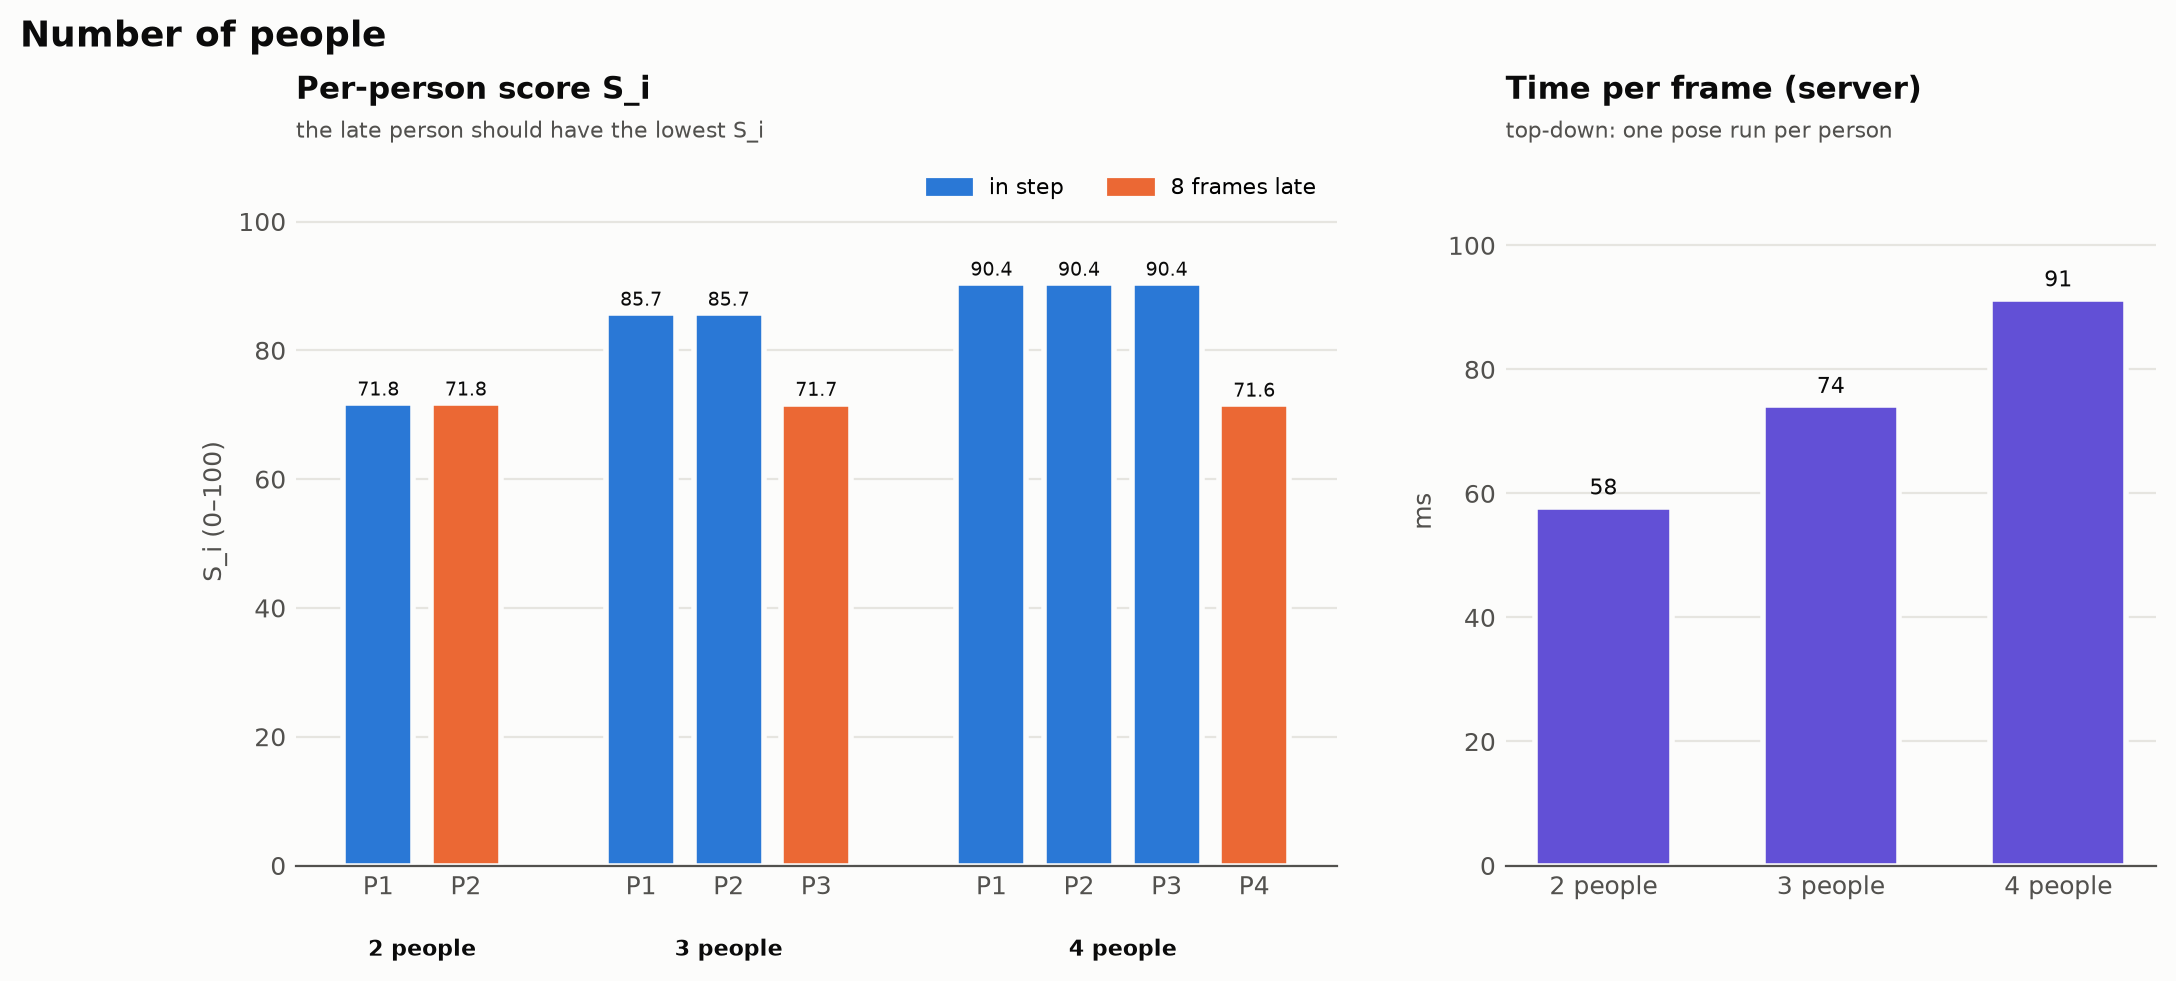
\includegraphics[width=\linewidth]{fig14_people}
\caption{Хүний тооноос хамаарах хүн тус бүрийн оноо болон нэг кадрын хугацаа}
\label{fig:fig14_people}
\end{figure}

\textbf{Шуугиан тэгшитгэлийн нөлөө.} Хүний тоо автоматаар зөв тоологдсон 30 хяналттай бичлэгийн оноог Савицкий-Голейн тэгшитгэлтэй болон тэгшитгэлгүйгээр тооцоолж харьцуулахад оноо дунджаар 0.59, хамгийн ихдээ 4.3 оноогоор зөрсөн. Тэгшитгэлгүй үед синхрон бичлэгүүдийн оноо 0.4--0.8 оноогоор буурсан бол өөр хөдөлгөөнтэй бичлэгүүдийнх 2.9--4.3 оноогоор буурсан бөгөөд хоцрогдлын үр дүн өөрчлөгдөөгүй. Энэхүү өндөр нягтаршилтай, тод бичлэгт гол цэгийн чичиргээ бага тул тэгшитгэлийн нөлөө бага гарсан. Чичиргээ ихтэй бичлэгт нөлөө нь илүү их байх төлөвтэй.

\textbf{Хоцрогдол оруулсан гол цэгийн түвшний туршилт.} Синхрончлол алдагдсан мөчийг хоцорсон хүн болон биеийн хэсгийн хамт зөв илрүүлж байгаа эсэхийг гол цэгийн түвшинд шалгав. Загвар сонголтын бичлэгийн нэг хүний бүх бие эсвэл нэг, хоёр мөчийн гол цэгийг 2.5--3 секундийн турш 0.3 эсвэл 0.5 секундээр хоцроож (t кадрын гол цэгийг тухайн хүний t − Δ кадрын гол цэгээр сольж), хоёр өөр хүн, хоёр өөр хугацаанд нийт 20 тохиолдол үүсгэв. Тохиолдол бүрт хоцроосон хугацаатай давхцсан, тухайн хүнийг агуулсан шинэ мөч илэрсэн, хоцорсон хүн болон мөчийг зөв нэрлэсэн эсэхийг шалгав (Хүснэгт~\ref{tab:delay_test}).

\begin{table}[H]
\centering
\caption{Хоцрогдол оруулсан гол цэгийн түвшний туршилтын үр дүн}
\label{tab:delay_test}
\small
\begin{tabular}{|>{\raggedright\arraybackslash}p{0.220\linewidth}|>{\raggedright\arraybackslash}p{0.140\linewidth}|>{\raggedright\arraybackslash}p{0.220\linewidth}|>{\raggedright\arraybackslash}p{0.280\linewidth}|}
\hline
\textbf{Хоцроосон хэсэг} & \textbf{Хоцрогдол} & \textbf{Зөв илрүүлсэн} & \textbf{Олдсон хоцрогдол (с)} \\ \hline
Бүх бие & 0.3 с & 2/2 & 0.48, 0.52 \\ \hline
Бүх бие & 0.5 с & 2/2 & 0.56, 0.68 \\ \hline
Хоёр гар & 0.3 с & 2/2 & 0.52, 1.08 \\ \hline
Хоёр гар & 0.5 с & 2/2 & 0.92, 1.32 \\ \hline
Баруун гар & 0.3 с & 2/2 & 0.68, 0.40 \\ \hline
Баруун гар & 0.5 с & 2/2 & 0.96, 0.60 \\ \hline
Хоёр хөл & 0.3 с & 2/2 & 0.28, 0.44 \\ \hline
Хоёр хөл & 0.5 с & 2/2 & 0.52, 0.60 \\ \hline
Зүүн хөл & 0.3 с & 0/2 & -- \\ \hline
Зүүн хөл & 0.5 с & 2/2 & 0.52, 0.56 \\ \hline
\textbf{Нийт} & & \textbf{18/20} & \\ \hline
\end{tabular}
\end{table}

20 тохиолдлын 18-д нь хоцорсон хүн болон мөчийг зөв илрүүлсэн бөгөөд илрүүлж чадаагүй хоёр тохиолдол хоёулаа нэг хөлийг 0.3 секундээр хоцроосон тохиолдол байв. Тухайн хугацаанд хөл бага хөдөлсөн үед хоцрогдол өнцгийн зөрүүнд бага нөлөөлдөг тул илрүүлэхэд хэцүү. Харин мөчийн түвшинд олдсон хоцрогдлын утга ихэнхдээ бодит хоцрогдлоос их гарсан (0.3 секундийг 0.28--1.08 секунд гэх мэт). Тулааны урлагийн хөдөлгөөн давтагддаг тул шилжилт нь мөчийг тухайн хөдөлгөөний өөр давталттай тааруулж болдог бөгөөд мөчийн хоцрогдлын хэмжээг тайлбарлахдаа үүнийг анхаарах шаардлагатай. Бүх биеийн хоцрогдлыг бүтэн бичлэгийн хувьд тооцоолоход (дээрх видеоны түвшний туршилт) ийм алдаа гараагүй.

\textbf{Хоцрогдлын онооны тогтворгүй байдал.} Гол цэгүүд бараг ижил (медиан 0.61 пиксел) байхад 4.3-ын хөтөч ба серверийн бүлгийн оноо 1.2 оноогоор, кадр бүрийн оноо 95-р перцентилээр 10.8 оноогоор зөрсөн. Бүрэлдэхүүн бүрээр задлан шинжлэхэд \(S_{pose}\) (медиан зөрүү 0.001) болон \(S_{corr}\) (0.003) бараг ижил байсан бол нийт 2568 цонхны 477-д нь \(S_{lag}\) өөр гарсан. Энэ бичлэгт цонхны \(\rho_{max}\)-ийн дундаж 0.44 буюу \(\rho_{min} = 0.3\) босгод ойрхон тул гол цэгийн өчүүхэн өөрчлөлт \(\rho_{max}\)-ийг босгоос дээш эсвэл доош гаргахад \(S_{lag}\) ойролцоогоор 0.9-өөс 0 руу огцом өөрчлөгддөг. Иймд босгын орчмын гурван хувилбарыг харьцуулав. Үүнд: одоогийн огцом босго (hard), босгын орчимд \(S_{lag}\)-ийг жигд өсгөх налуу (ramp), \(\rho_{max} < \rho_{min}\) үед хоцрогдлыг «хэмжигдээгүй» гэж үзэн онооноос хасах (drop). Налуу хувилбарт

\begin{equation}
S_{lag} = \max\left(0, \; 1 - \frac{|\tau^{*}|}{\tau_{max}}\right) \cdot \min\left(1, \; \max\left(0, \; \frac{\rho_{max} - (\rho_{min} - w/2)}{w}\right)\right)
\end{equation}

бөгөөд \(w = 0.2\) үед \(S_{lag}\) нь \(\rho_{max} = 0.2\)-оос 0.4 хүртэл 0-ээс одоогийн утга хүртэл жигд өснө. Хувилбар бүрийг тогтвортой байдал (ижил бичлэгийн хөтөч ба серверийн ажиллуулалтын онооны зөрүү) болон ялгах чадвар (2-р хүнийг гол цэгийн түвшинд 0.12--0.8 секундээр хоцроох, эсвэл тухайн хүний 7 болон 13 секундийн зайтай өөр хэсгийн хөдөлгөөнөөр солиход 1--2 хосын оноо зөв дарааллаар буурч байгаа эсэх) гэсэн хоёр шалгуураар үнэлэв (Хүснэгт~\ref{tab:lag_variants}, Зураг~\ref{fig:fig9_lag_confidence}).

\begin{table}[H]
\centering
\caption{Хоцрогдлын онооны хувилбаруудын харьцуулалт}
\label{tab:lag_variants}
\small
\begin{tabular}{|>{\raggedright\arraybackslash}p{0.120\linewidth}|>{\raggedright\arraybackslash}p{0.180\linewidth}|>{\raggedright\arraybackslash}p{0.180\linewidth}|>{\raggedright\arraybackslash}p{0.400\linewidth}|}
\hline
\textbf{Хувилбар} & \textbf{Бүлгийн онооны зөрүү} & \textbf{Кадр бүрийн зөрүү (95-р перцентиль)} & \textbf{1--2 хосын оноо: синхрон / 0.12 / 0.2 / 0.4 / 0.8 с хоцрогдол / өөр хөдөлгөөн (7 с, 13 с)} \\ \hline
hard & 1.21 & 10.75 & 82.8 / 77.9 / 73.8 / 65.9 / 54.1 / 48.1, 46.8 \\ \hline
ramp 0.2 & 0.39 & 5.10 & 83.4 / 78.2 / 74.1 / 66.1 / 54.0 / 48.7, 47.5 \\ \hline
ramp 0.4 & 0.11 & 4.43 & 82.1 / 77.2 / 73.2 / 65.4 / 53.6 / 50.3, 50.7 \\ \hline
drop & 0.09 & 2.05 & 88.1 / 82.9 / 78.7 / 70.5 / 63.2 / 66.0, 68.0 \\ \hline
\end{tabular}
\end{table}

\begin{figure}[H]
\centering
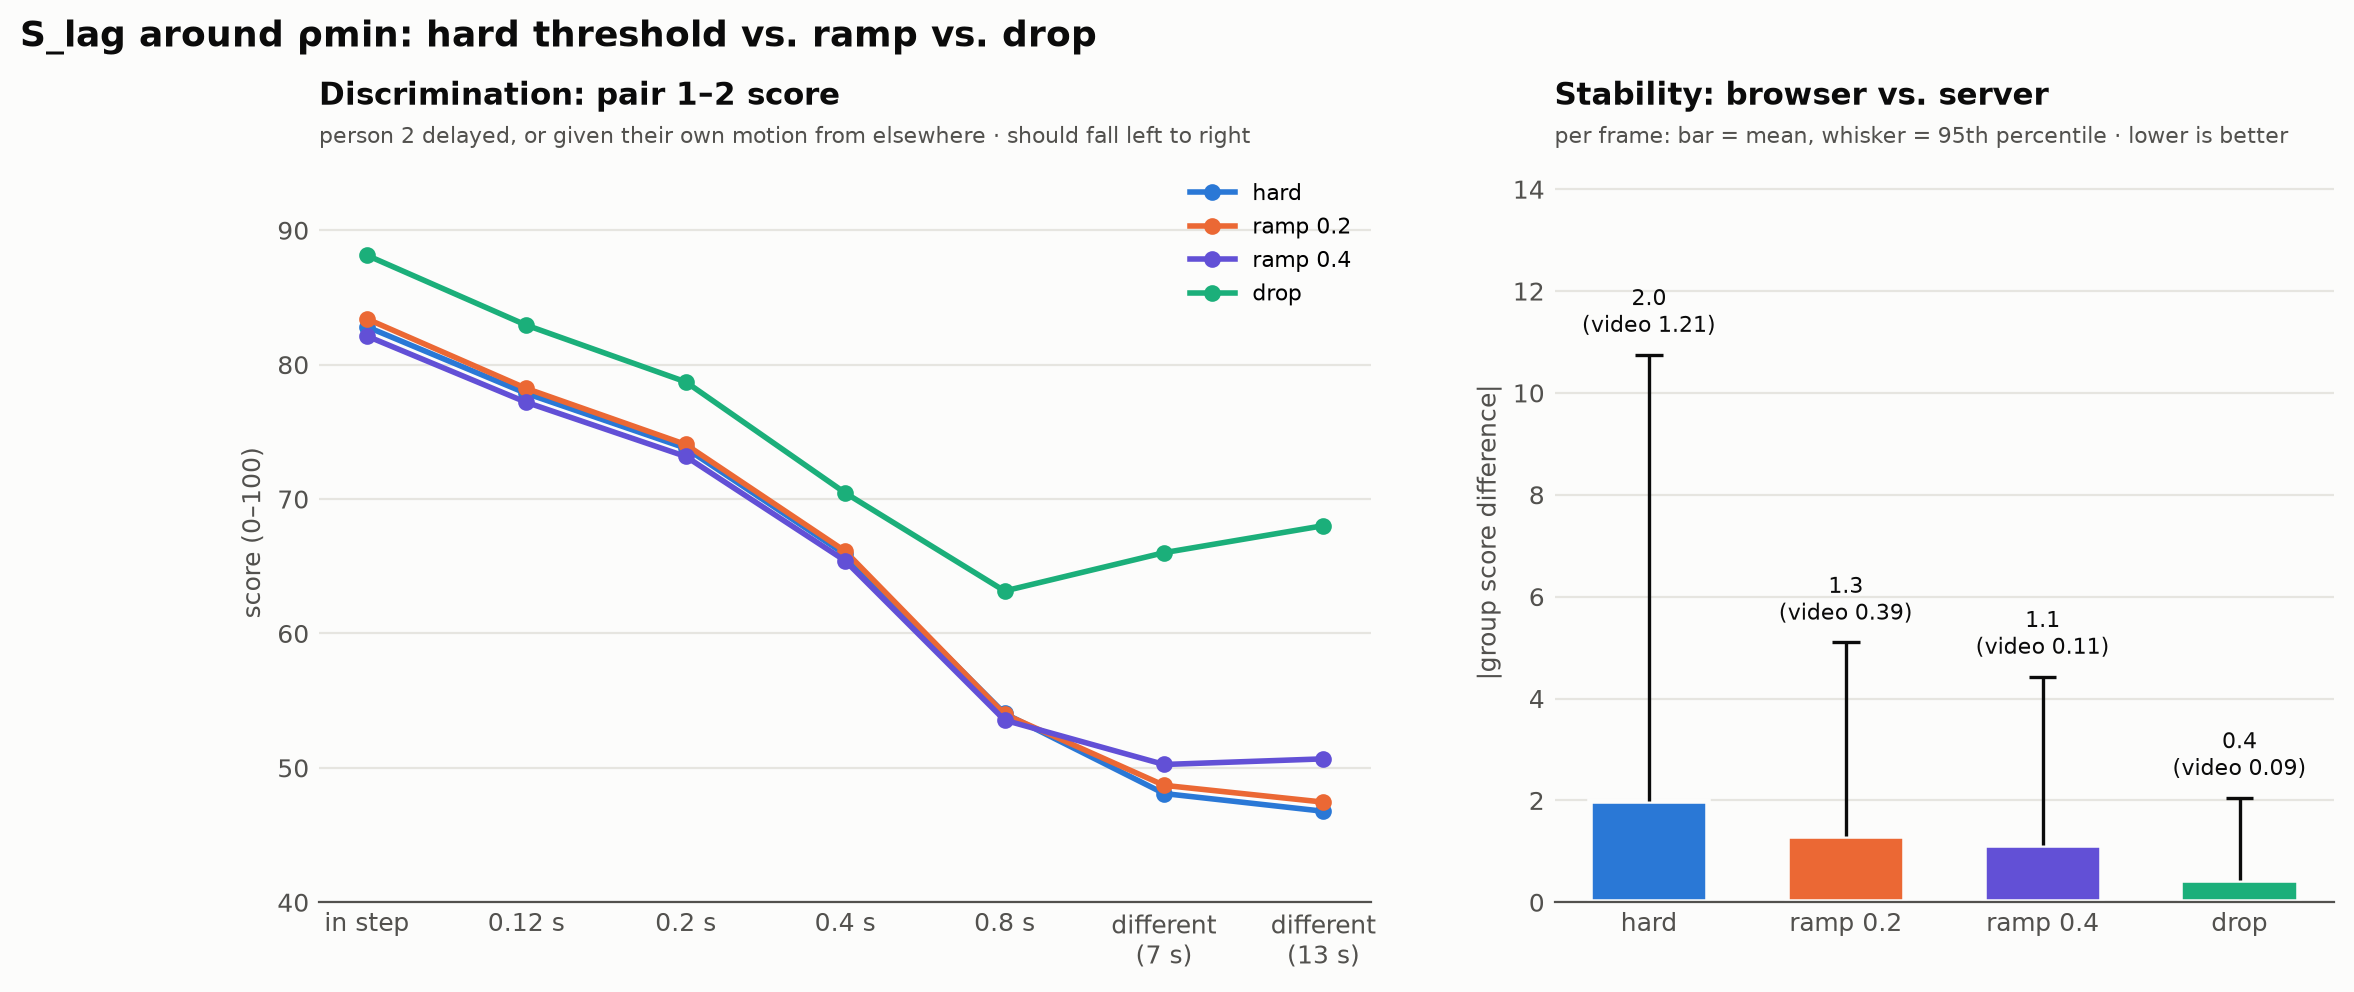
\includegraphics[width=\linewidth]{fig9_lag_confidence}
\caption{Хоцрогдлын онооны хувилбаруудын ялгах чадвар ба тогтвортой байдал}
\label{fig:fig9_lag_confidence}
\end{figure}

Хасах (drop) хувилбар хамгийн тогтвортой боловч өөр хөдөлгөөнд (66--68) 0.8 секундийн хоцрогдлоос (63.2) илүү өндөр оноо өгч байгаа тул ашиглах боломжгүй. Учир нь хоцрогдлыг хэмжих боломжгүй байх нь синхрон бус байгаагийн шинж бөгөөд түүнийг онооноос хасах нь торгуулийг арилгаж байна. Налуу хувилбарын \(w = 0.4\) нь илүү тогтвортой ч \(\rho_{max} \approx 0.1\) буюу бараг хамааралгүй цонхонд ч \(S_{lag}\) өгдөг тул өөр хөдөлгөөний оноо өсч, ялгах чадвар буурсан. Харин \(w = 0.2\) нь бүлгийн онооны зөрүүг 3 дахин (1.21-ээс 0.39), кадр бүрийн зөрүүг 2 дахин бууруулж, ялгах чадвар нь одоогийн хувилбартай бараг ижил хэвээр байна. Мөн түүний муж (0.2--0.4) нь өөр хөдөлгөөний (0.13) болон хамт хөдөлж буй хүмүүсийн (0.42) \(\rho_{max}\)-ийн медиануудын хооронд оршдог. Хүний тоо автоматаар зөв тоологдсон 30 хяналттай бичлэг дээр налуу хувилбарын оноо анхдагч хувилбарынхаас дунджаар 0.11, хамгийн ихдээ 2.4 оноогоор зөрсөн бөгөөд нөхцлүүдийн дараалал өөрчлөгдөөгүй. Иймд \(w = 0.2\) налуу хувилбарыг ашиглахыг санал болгож байна. Энэ бүлгийн бусад бүх үр дүнг анхдагч огцом босгоор (hard) тооцоолсон. Кадр бүрийн онооны үлдсэн зөрүү (95-р перцентиль 5.1) нь хөндлөн корреляцын хоёр ойролцоо оргилын хооронд \(\tau^{*}\) үсрэхээс үүдэлтэй.

\headshort{Бодит бичлэг}
\section{Бодит бичлэг дээрх туршилт}

\textbf{Тулааны урлагийн бичлэг.} Загвар сонголтын бичлэгт гурван хүн тулааны урлагийн ижил хөдөлгөөнийг хамтдаа хийдэг. Синхрончлолын алгоритмаар бүлгийн оноо 82.6 гарав (Хүснэгт~\ref{tab:sync_result}).

\begin{table}[H]
\centering
\caption{Тулааны урлагийн бичлэгийн синхрончлолын үр дүн}
\label{tab:sync_result}
\small
\begin{tabular}{|>{\raggedright\arraybackslash}p{0.130\linewidth}|>{\raggedright\arraybackslash}p{0.090\linewidth}|>{\raggedright\arraybackslash}p{0.090\linewidth}|>{\raggedright\arraybackslash}p{0.090\linewidth}|>{\raggedright\arraybackslash}p{0.090\linewidth}|>{\raggedright\arraybackslash}p{0.180\linewidth}|>{\raggedright\arraybackslash}p{0.120\linewidth}|}
\hline
\textbf{Хос} & \textbf{Оноо} & \textbf{Гар} & \textbf{Хөл} & \textbf{Их бие} & \textbf{Хоцрогдол (\(\rho_{max}\))} & \textbf{Толин тусгал} \\ \hline
1--2 & 83.6 & 81.8 & 90.4 & 86.6 & 0 с (0.31) & 0.4\% \\ \hline
1--3 & 79.5 & 77.3 & 81.7 & 79.9 & 0.08 с (0.23) & 11.6\% \\ \hline
2--3 & 84.6 & 80.8 & 86.1 & 87.0 & 0.04 с (0.28) & 5.8\% \\ \hline
\end{tabular}
\end{table}

Хүн тус бүрийн оноо \(S_1 = 81.6\), \(S_2 = 84.1\), \(S_3 = 82.0\) бөгөөд 1-р хүн бүлгээсээ хамгийн их зөрж байна. Бүх хосод гарын оноо хамгийн бага байгаа нь хурдан хөдөлдөг, чичиргээ ихтэй бугуйн цэгүүдтэй (3.2) уялдана. Бүх бичлэгийн хоцрогдлын хувьд 1--3 болон 2--3 хосын \(\rho_{max}\) нь \(\rho_{min} = 0.3\)-аас бага тул тэдгээрт итгэхгүй. Кадр бүрийн онооны графикаас (Зураг~\ref{fig:fig8_sync_timeline}) бичлэгийн эхний 20 секундэд бүлгийн оноо ихэвчлэн 85--93 байхад 20-оос хойш хэд хэдэн удаа 60--66 хүртэл буурч байгааг харж болно. Алгоритм нийт 12 синхрончлол алдагдсан мөч илрүүлсэн бөгөөд тэдгээрийн ихэнх нь гарын хоцрогдол байв.

\begin{figure}[H]
\centering
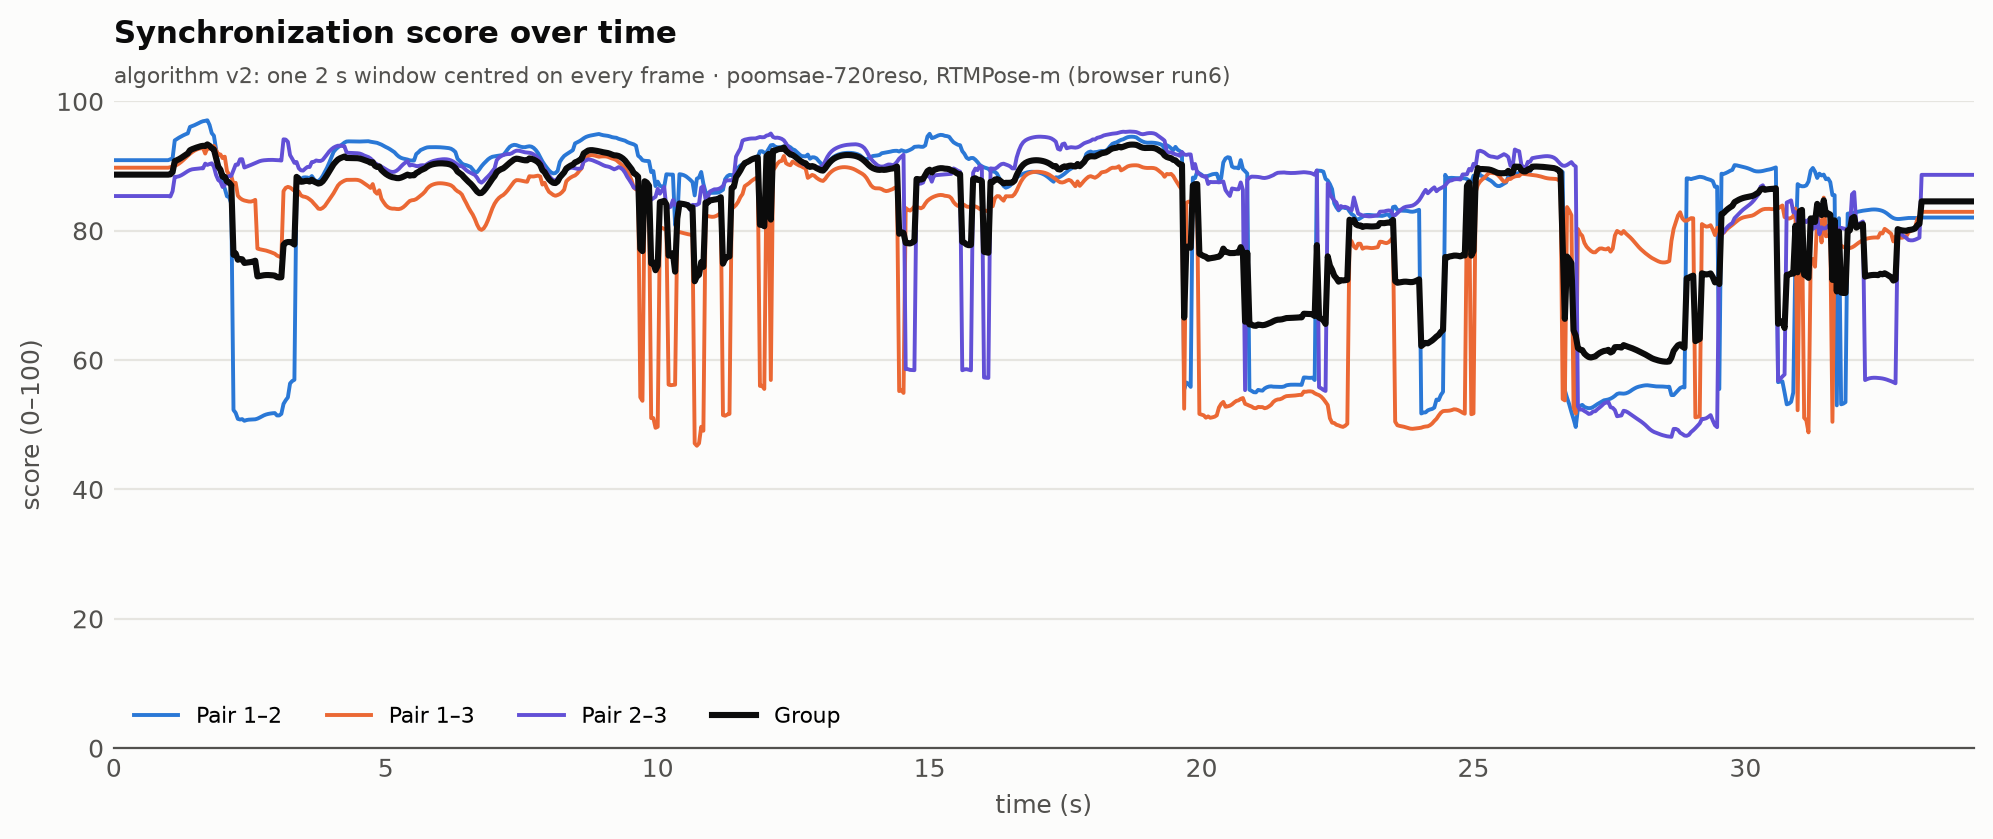
\includegraphics[width=\linewidth]{fig8_sync_timeline}
\caption{Бүлгийн болон хос бүрийн синхрончлолын оноо (кадр бүрээр)}
\label{fig:fig8_sync_timeline}
\end{figure}

\textbf{Бүжгийн бичлэгүүд.} Гурван бүжигчин ижил бүжгийг хамтдаа бүжиглэсэн дөрвөн бичлэгийн үр дүнг Хүснэгт~\ref{tab:real}-д нэгтгэв.

\begin{table}[H]
\centering
\caption{Гурван хүнтэй бүжгийн бичлэгүүдийн синхрончлолын үр дүн}
\label{tab:real}
\small
\begin{tabular}{|>{\raggedright\arraybackslash}p{0.100\linewidth}|>{\raggedright\arraybackslash}p{0.090\linewidth}|>{\raggedright\arraybackslash}p{0.140\linewidth}|>{\raggedright\arraybackslash}p{0.090\linewidth}|>{\raggedright\arraybackslash}p{0.190\linewidth}|>{\raggedright\arraybackslash}p{0.110\linewidth}|>{\raggedright\arraybackslash}p{0.090\linewidth}|}
\hline
\textbf{Бичлэг} & \textbf{Урт (с)} & \textbf{Гурван хүн илэрсэн кадр} & \textbf{Бүлгийн оноо} & \textbf{\(S_1 / S_2 / S_3\)} & \textbf{Нэг кадрын хугацаа (мс)} & \textbf{Зөрсөн мөч} \\ \hline
1 & 42.6 & 93.1\% & 69.4 & 68.1 / 71.2 / 68.8 & 71.6 & 15 \\ \hline
2 & 42.6 & 86.0\% & 67.0 & 67.5 / 67.7 / 65.7 & 70.6 & 16 \\ \hline
3 & 34.9 & 86.4\% & 71.2 & 71.6 / 71.8 / 70.2 & 62.3 & 13 \\ \hline
4 & 30.7 & 98.3\% & 79.1 & 80.6 / 77.0 / 79.8 & 72.0 & 9 \\ \hline
\end{tabular}
\end{table}

Бодит бүжигчдийн бүлгийн оноо 67.0--79.1 буюу нэг хүний хуулбартай синхрон бичлэгийнхээс (99.8) мэдэгдэхүйц бага, харин өөр хөдөлгөөний онооноос (45.4--62.0) их гарсан. Энэ нь ижил бүжгийг хамтдаа бүжиглэсэн ч хүмүүсийн хөдөлгөөний далайц, хэлбэр, хэмнэлд байгалийн зөрүү байдагтай нийцнэ. Бичлэгүүдийн бүх бичлэгийн \(\rho_{max}\) 0.13--0.35 хооронд байсан бөгөөд ихэнх хосод \(\rho_{min} = 0.3\)-аас бага тул бүх бичлэгийн хоцрогдлыг найдвартай гэж үзээгүй. Бүжигчид бие биеийнхээ урдуур, хойгуур шилжиж халхалдаг тул гурван хүн бүгд илэрсэн кадрын хувь 86.0--98.3\% байсан ба дутуу кадруудыг 3.4-ийн аргаар нөхсөн. Хамгийн өндөр оноотой 4-р бичлэгт хосуудын хөлийн оноо 85.3--88.9 байхад гарын оноо 62.8--76.1 байсан нь бүжигчдийн гарын хөдөлгөөн хөлийнхөөс илүү зөрж байгааг харуулна. Бүжигчдийн синхрончлолын жинхэнэ түвшин тэмдэглэгдээгүй тул эдгээр оноо зөв эсэхийг шүүгчийн үнэлгээтэй харьцуулж баталгаажуулах шаардлагатай.

\textbf{Загвар бүрийн нягтаршлын нөлөө.} Загвар сонголтын шатанд тулааны урлагийн бичлэгийг 360p, 480p, 720p нягтаршилтай хувилбараар таван загвараар боловсруулж, 720p-ийн үр дүнтэй харьцуулсан (Зураг~\ref{fig:fig10_resolution}). RTMPose-m бүх нягтаршилд кадрын 100\%-д гурван хүнийг бүгдийг нь илрүүлж, 720p-ийн гол цэгээс хүрээний өндрийн 5\%-ийн дотор байсан гол цэгийн хувь 480p-д 98.6\%, 360p-д 94.5\% байв. MediaPipe-ийн хувьд 68\% ба 75\% байсан нь нягтаршилд хамгийн мэдрэмтгий байв. Энэ туршилтыг кадр унших алдааг засахаас өмнө 30 кадр/с давтамжаар хийсэн боловч хяналттай бичлэг дээрх нягтаршлын туршилт (4.4) нь RTMPose-m-ийн хувьд ижил дүгнэлтэд хүрсэн.

\begin{figure}[H]
\centering
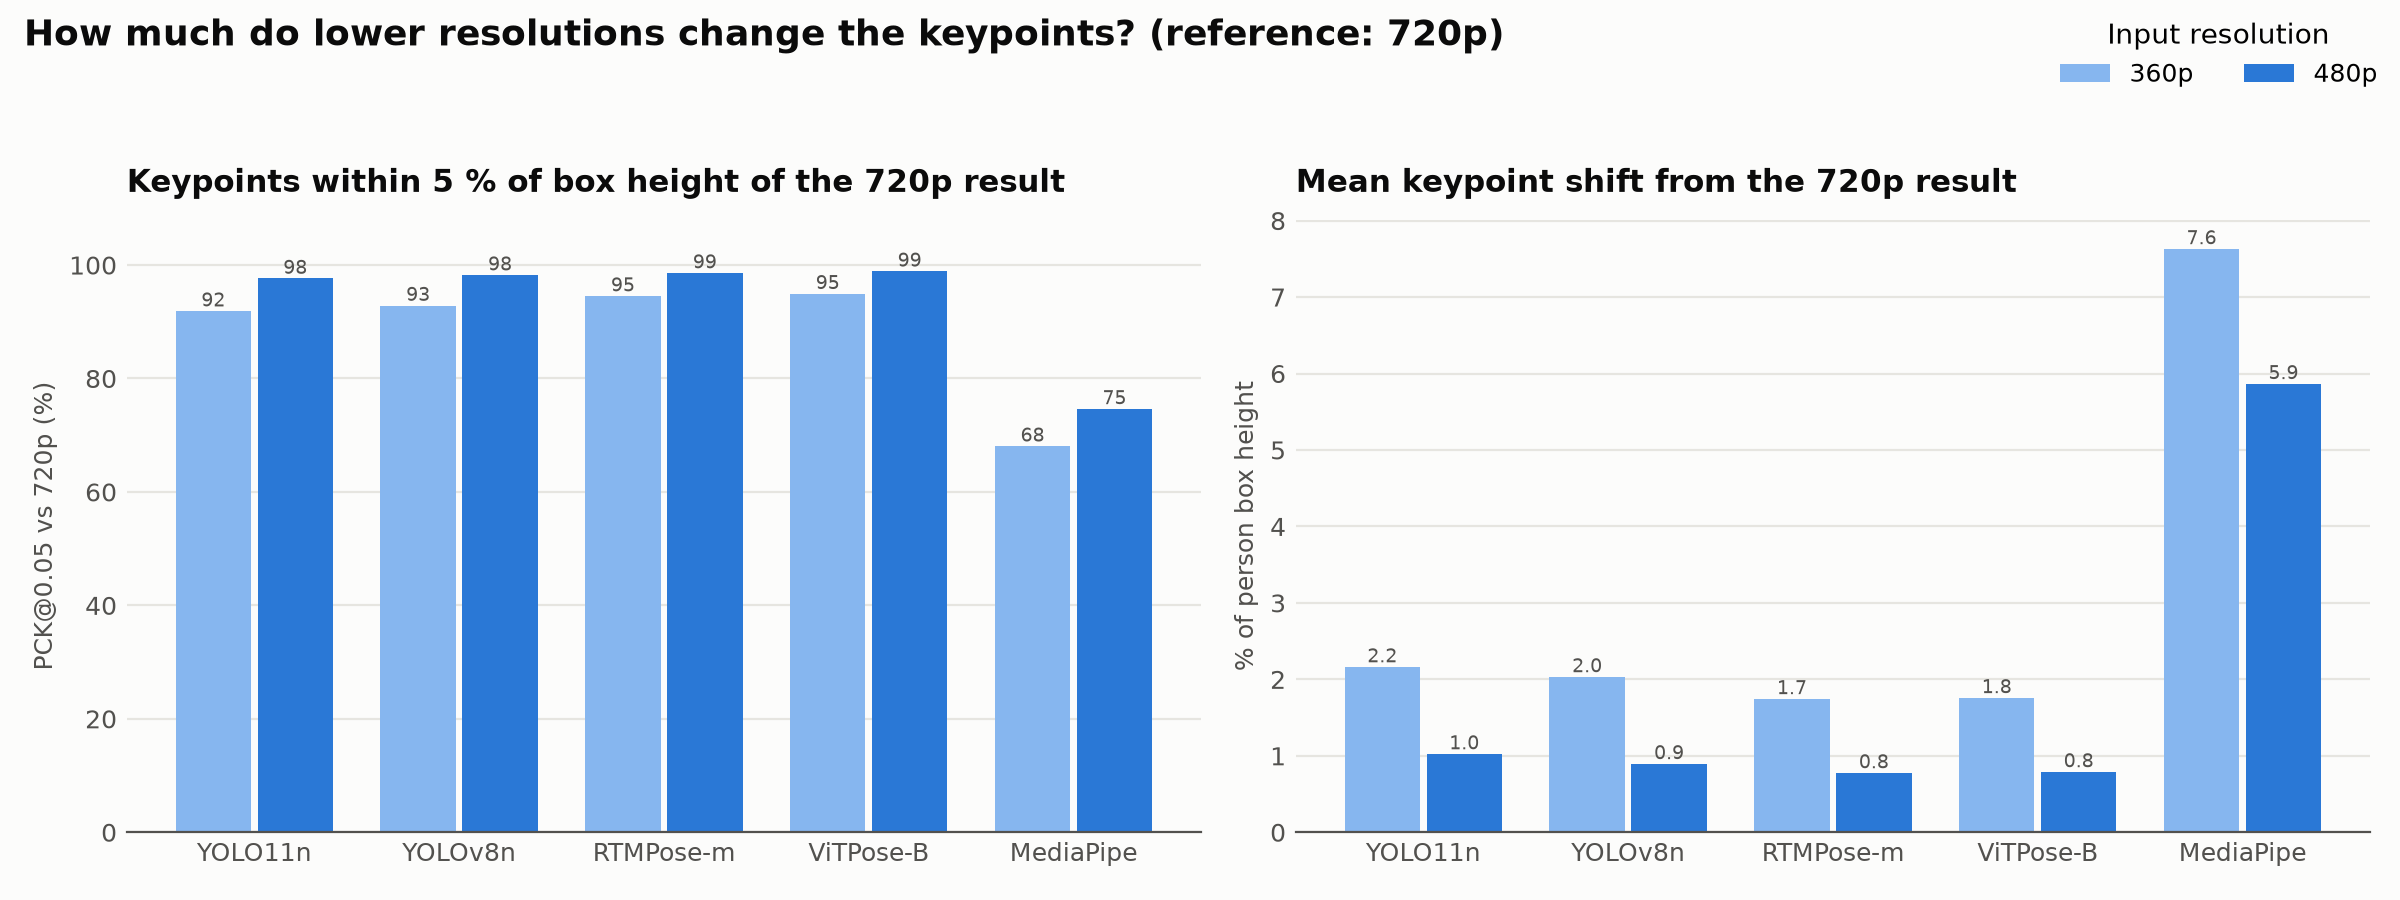
\includegraphics[width=\linewidth]{fig10_resolution}
\caption{Бага нягтаршилд гол цэгийн 720p-ийн үр дүнтэй тохирох байдал ба дундаж шилжилт}
\label{fig:fig10_resolution}
\end{figure}

\section{Аргын хязгаарлалт}

Туршилтын үр дүнд үндэслэн аргын дараах хязгаарлалтыг тодорхойлов. Үүнд:

\begin{itemize}
\item
  Хүний тоог эхний 2 секундийн илрүүлэлтээр автоматаар тодорхойлдог тул хүний өндөр ойролцоогоор 140 пикселээс бага эсвэл бичлэгийн нягтаршил 240p ба түүнээс бага үед хүний тоо буруу тоологдож болно. Энэ үед хэрэглэгч хүний тоог гараар өгөх шаардлагатай.
\item
  Ойролцоогоор 1 секунд ба түүнээс их хоцрогдол оноогоороо өөр хөдөлгөөнтэй ижил түвшинд хүрдэг тул тэдгээрийг ялгахдаа бүх бичлэгийн хоцрогдол ба \(\rho_{max}\)-ийг хамт харах шаардлагатай.
\item
  Мөчийн түвшний хоцрогдлын хэмжээ давтагддаг хөдөлгөөнд бодит утгаасаа их гарч болох бөгөөд бага хөдөлж буй мөчийн (жишээлбэл, 0.3 секундийн хөлийн) хоцрогдлыг илрүүлэх боломжгүй.
\item
  Хоцрогдлын оноо \(\rho_{min}\) босгын орчимд огцом өөрчлөгддөг тул гол цэгийн өчүүхэн ялгаа кадр бүрийн оноонд мэдэгдэхүйц нөлөөлдөг. Налуу хувилбар энэ нөлөөг бууруулна.
\item
  Үений өнцгийг 2D зураг дээр тооцоолдог тул хүмүүс камерт ойролцоо ижил чиглэлээр харсан байх шаардлагатай. Мөн хүмүүс байраа солихгүй, бие биеэ удаан хугацаанд бүрэн халхлахгүй гэж үзсэн.
\item
  Хяналттай өгөгдөл нь нэг хүний бичлэгийн хуулбар тул бодит хүмүүсийн хооронд байдаг хөдөлгөөний байгалийн зөрүү, биеийн хэмжээ, хувцасны ялгааг агуулаагүй. Бодит бичлэгүүдийн синхрончлолын жинхэнэ түвшин тэмдэглэгдээгүй тул бодит бичлэг дээрх үр дүнг шүүгчийн үнэлгээтэй харьцуулаагүй.
\item
  Биеийн хэсгийн жин болон нэгдсэн онооны жингүүдийг (\(w_1 = w_2 = w_3\)) судлаач тогтоосон бөгөөд өгөгдөлд суурилан тохируулаагүй.
\end{itemize}
